\chapter{Działanie systemu}
Działanie systemu zostanie zaprezentowane w oparciu o kilka przykładów. Dla każdego przykładu przedstawione zostały grafy z zaznaczonymi ścieżkami, które zostały wybrane podczas etapu udzielania odpowiedzi. Odpowiedzi na pytania są także przedstawione w formie tekstowej. Następnie, dla każdego przykładu przedstawiono listę konfliktów, które mogą wystąpić oraz zmiany, jakie należy wprowadzić w przypadku ich wystąpienia. Węzły grafów posiadają etykiety, które zawierają na końcu w nawiasach identyfikatory swoich węzłów. Identyfikatory te są używane przy opisie konfliktów oraz zmian. Pogrubioną czcionką zaznaczono znalezione konflikty.
% SW: W obecnej formie ta sekcja jest bardzo skrótowa. Powinien Pan w "rozbiegówce" wyjaśnić, że pokaże Pan działanie systemu na kilku przykładach. Większość to rzeczywiste wytyczne (uproszczone na potrzeby testowania. Wykorzystywane są też przykłady sztuczne demonstrujące zachowanie algorytmu w granicznych wypadkach (tutaj chodzi mi o przykład, gdzie w ramach usuwania jednego konfliktu wprowadzanych jest kilka zmian). Jeśli natomiast chodzi o przykłady rzeczywiste, to dodałbym także przykład z dawkami leków -- brakuje go do pełnej demonstracji Pana dokonań.

% SW: Również na wstępie powinien Pan wyjaśnić, że opisując poszczególne przykłady pokaże Pan rozważane wytyczne w formie grafów z zaznaczonymi ścieżkami odpowiadającymi dostępnym danym pacjenta, dostępną wiedzę na temat konfliktów i sposobów ich rozwiązania, a także wynikowe grafy (a przynajmniej ich zmodyfikowane fragmenty). Przedstawiając konflikty powinien zaznaczyć Pan te, które zostały wykryte i usunięte dla danego pacjenta. Wreszcie konflikty i sposoby ich usunięcia powinien Pan przedstawić korzystając ze składni, którą Pan zaproponował (jest to bardzo eleganckie rozwiązanie i warto się nim pochwalić).

\section{Przypadek 1 - atak astmy i wrzód trawienny}
Wytyczne dla ataku astmy (ang. \textit{asthma exacerbation}) przedstawiono na rys. \ref{fig:ag_ae}.\\*
Wytyczne dla wrzodu trawiennego (ang. \textit{peptic ulcer}) przedstawiono na rys. \ref{fig:pu}.

% SW: Każdy graf, zestaw danych pacjenta oraz lista konfliktów powinien zostac potraktowany jako rysunek z numerem i tytułem (wprowadziłem odpowiednią zmianę poniżej), a w tekście powinno się do niego znaleźć odwołanie).

% SW: Warto byłoby ujednolicić wszystkie diagramy, aby w wierzchołku kontekstowym pojawiał sie zawsze akronim lub nazwa choroby. Obecnie mamy albo choroby, albo zdania "Patient diagnosed with ...".  
\begin{figure}[H]
\centering
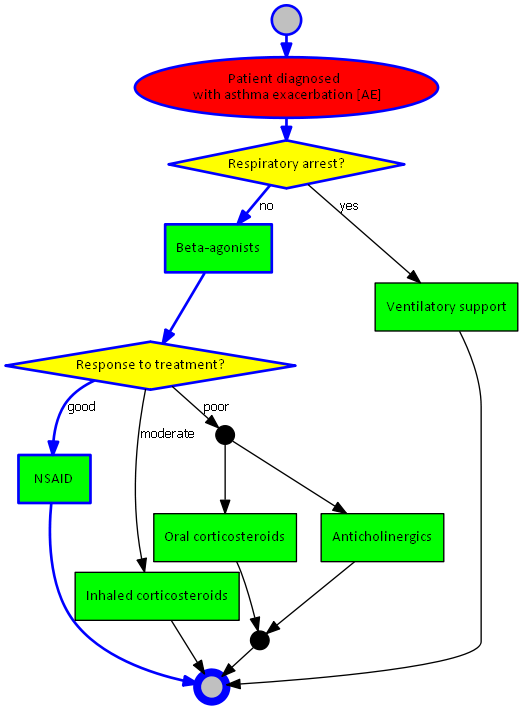
\includegraphics[scale=0.5]{img/asthma.png}
\caption{Wytyczne dla ataku astmy}
\label{fig:ag_ae}
\end{figure}

\newpage
\begin{figure}[H]
\centering
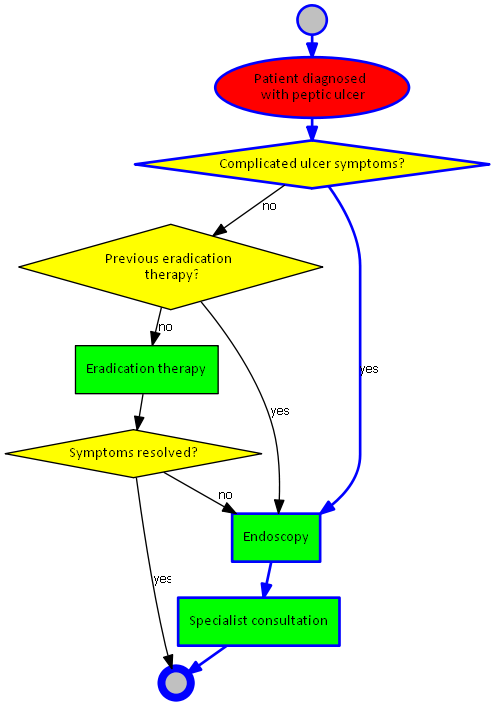
\includegraphics[scale=0.5]{img/peptic-ulcer.png}
\caption{Wytyczne dla wrzodu trawiennego}
\label{fig:pu}
\end{figure}
\newpage
\noindent Odpowiedzi na pytania:
\begin{enumerate}
\item{Atak astmy:
	\begin{itemize}
	\item{Respiratory arrest?: no}
	\item{Response to treatment?: good}
	\end{itemize}
}
\item{Wrzód trawienny:
	\begin{itemize}
	\item{Complicated ulcer symptoms?: yes}
	\end{itemize}
}
\end{enumerate}
Konflikty:\\*
c\_pe a\_oral\_cortico:replace a\_oral\_cortico with a\_inh\_cortico2\\*
\textbf{c\_pe a\_nsaid:add ppi after a\_nsaid}\\*
a\_et a\_inh\_cortico:replace a\_inh\_cortico with a\_oral\_cortico2
\newpage
\section{Przypadek 2 - migotanie przedsionków, przewlekła choroba nerek i nadciśnienie}
Wytyczne dla migotania przedsionków (ang. \textit{atrial fibrillation}) przedstawiono na rys. \ref{fig:afib}.\\*
Wytyczne dla przewlekłej choroby nerek (ang. \textit{chronic kidney disease}) przedstawiono na rys. \ref{fig:htn}.\\*
Wytyczne dla nadciśnienia (ang. \textit{hypertension}) przedstawiono na rys. \ref{fig:htn}.
\begin{figure}[H]
\centering
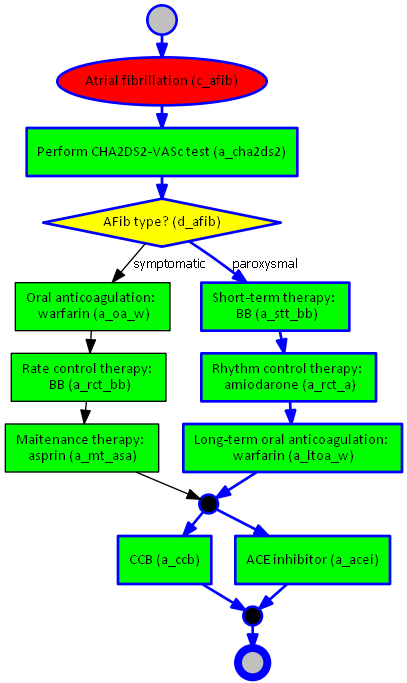
\includegraphics[scale=0.5]{img/afib-ver-4.png}
\caption{Wytyczne dla migotania przedsionków}
\label{fig:afib}
\end{figure}
\newpage
\begin{figure}[H]
\centering
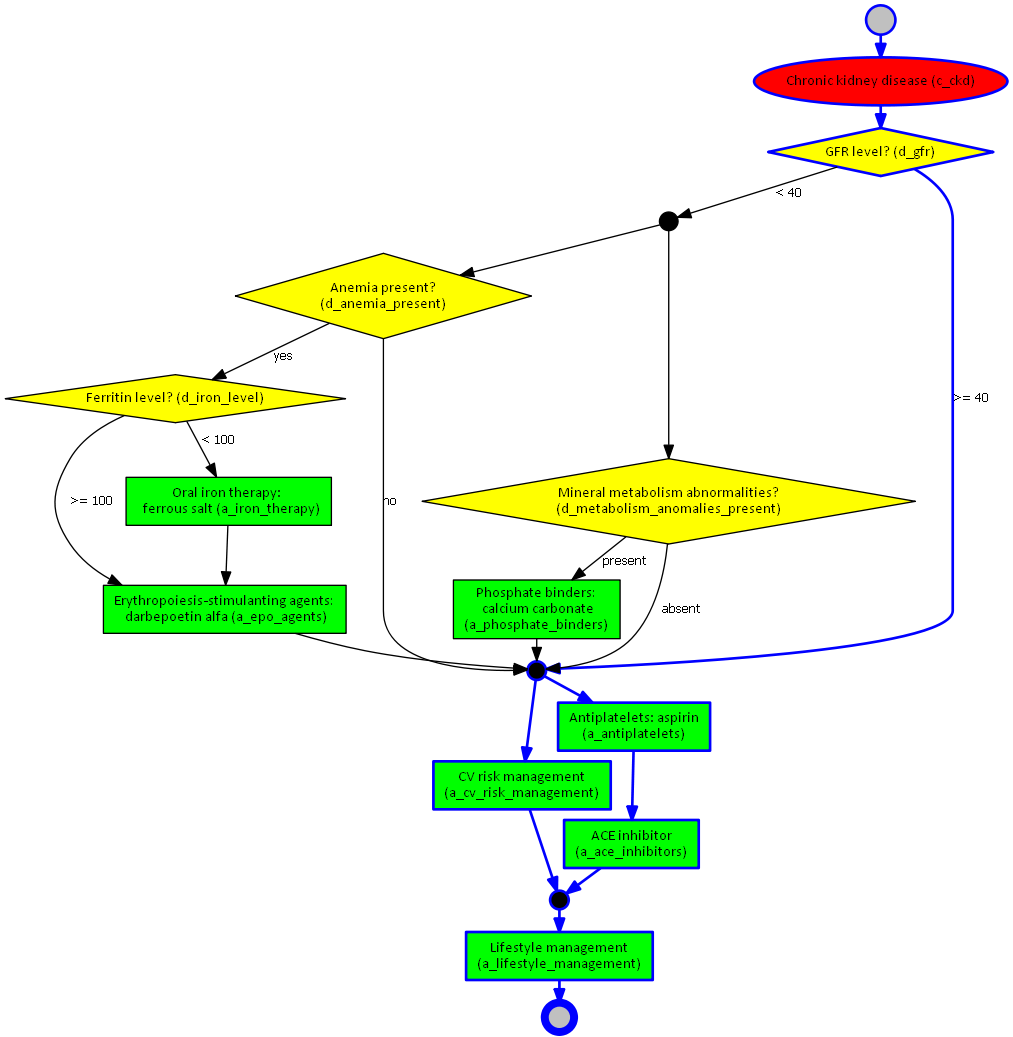
\includegraphics[scale=0.4]{img/ckd-simplified-ver-5.png}
\caption{Wytyczne dla przewlekłej choroby nerek}
\label{fig:ckd}
\end{figure}
\newpage
\begin{figure}[H]
\centering
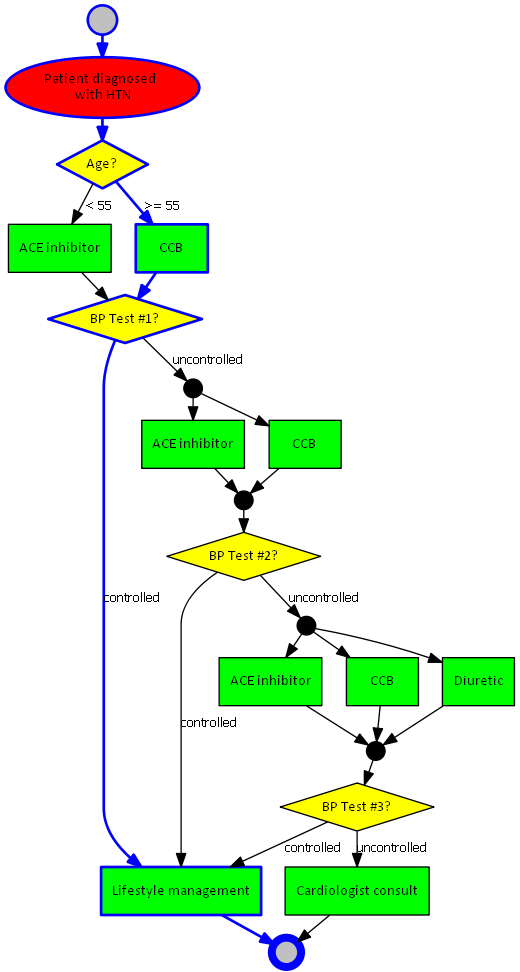
\includegraphics[scale=0.5]{img/htn-ver-3.png}
\caption{Wytyczne dla nadciśnienia}
\label{fig:htn}
\end{figure}
\newpage
\noindent Odpowiedzi na pytania:
\begin{enumerate}
\item{Migotanie przedsionków:
	\begin{itemize}
	\item{AFib type?: paroxysmal}
	\end{itemize}
}
\item{Przewlekła choroba nerek:
	\begin{itemize}
	\item{GFR level?: >=40}
	\end{itemize}
}
\item{Nadciśnienie:
	\begin{itemize}
	\item{Age?: >=55}
	\item{BP Test \#1?: controlled}
	\end{itemize}
}
% SW: Tutaj warto zaznaczyć, że te dane (to pytanie) nie pojawiają się jawnie w żadnych rozważanych wytycznych, ale są uwzględnione podczas sprawdzania konfliktów, dlatego użytkownik jest proszony o podanie odpowiedniej wartości.
\item{CHA2DS2-VASc = 5 (Parametr ten nie pojawia się jawnie w wytycznych, użytkownik jest proszony o podanie tej wartości)}
\end{enumerate}
Konflikty:\\*
\textbf{c\_htn c\_ckd:remove a\_step1\_acei,remove a\_step1\_ccb}\\*
\textbf{c\_afib c\_ckd c\_htn:remove a\_step3\_diuretric}\\*
\textbf{c\_afib c\_ckd:replace a\_antiplatelets with warfarin,replace a\_rct\_a with BB}\\*
\textbf{c\_afib c\_ckd \&CHA2DS2-VASc>2:replace a\_mt\_asa with warfarin2}\\*
c\_afib c\_ckd \&CHA2DS2-VASc<=1:replace a\_oa\_w with aspirin1,replace a\_ltoa\_w with aspirin2
\newpage
\section{Przypadek 3 - wrzód dwunastnicy i przemijający atak niedokrwienny}
Wytyczne dla wrzodu dwunastnicy (ang. \textit{duodenal ulcer}) przedstawiono na rys. \ref{fig:du}.\\*
Wytyczne dla przemijającego ataku niedokrwiennego (ang. \textit{transient ischemic attack}) przedstawiono na rys. \ref{fig:tia}.
\begin{figure}[H]
\centering
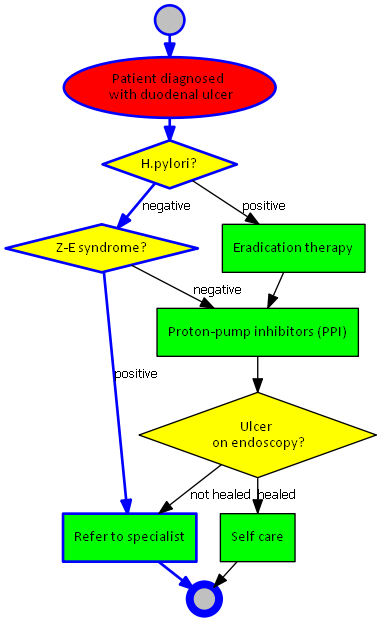
\includegraphics[scale=0.5]{img/du.png}
\caption{Wytyczne dla wrzodu dwunastnicy}
\label{fig:du}
\end{figure}
\newpage
\begin{figure}[H]
\centering
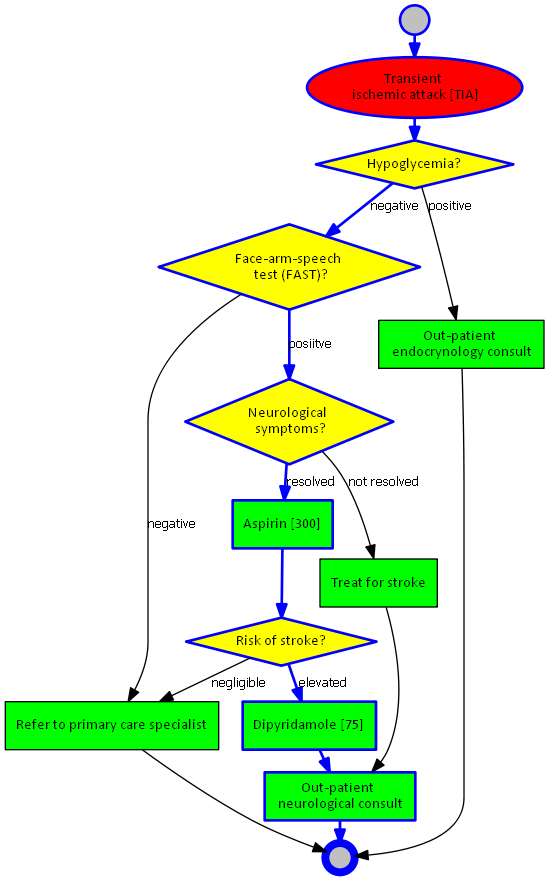
\includegraphics[scale=0.5]{img/tia.png}
\caption{Wytyczne dla przemijającego ataku niedokrwiennego}
\label{fig:tia}
\end{figure}
\newpage
\noindent Odpowiedzi na pytania:
\begin{enumerate}
\item{Wrzód dwunastnicy:
	\begin{itemize}
	\item{H.pylori?: negative}
	\item{Z-E syndrome?: positive}
	\end{itemize}
}
\item{Przemijający atak niedokrwienny:
	\begin{itemize}
	\item{Hypoglycemia?: negative}
	\item{Face-arm-speech test (FAST)?: positive}
	\item{Neurological symptoms?: resolved}
	\item{Risk of stroke?: elevated}
	\end{itemize}
}
\end{enumerate}
Konflikty:\\*
c\_du a\_aspirin not(a\_ppi) not(a\_dipyridamole):replace a\_aspirin with cl\\*
\textbf{c\_du a\_aspirin not(a\_ppi) a\_dipyridamole:add a\_ppi2 after d\_ze\_syndrome?positive, decrease\_dosage a\_aspirin 50}
